


\tikzset{every picture/.style={line width=0.75pt}} %set default line width to 0.75pt        

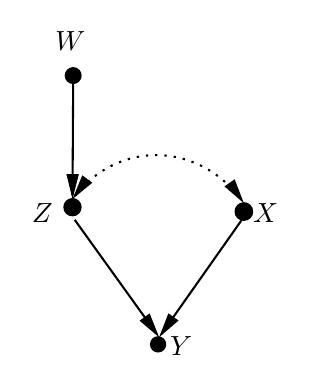
\begin{tikzpicture}[x=0.75pt,y=0.75pt,yscale=-1,xscale=1]
%uncomment if require: \path (0,300); %set diagram left start at 0, and has height of 300

%Shape: Circle [id:dp29577051361470774] 
\draw  [fill={rgb, 255:red, 0; green, 0; blue, 0 }  ,fill opacity=1 ] (85.5,142.67) .. controls (85.5,140.5) and (87.25,138.75) .. (89.42,138.75) .. controls (91.58,138.75) and (93.33,140.5) .. (93.33,142.67) .. controls (93.33,144.83) and (91.58,146.58) .. (89.42,146.58) .. controls (87.25,146.58) and (85.5,144.83) .. (85.5,142.67) -- cycle ;
%Shape: Circle [id:dp8954921583711406] 
\draw  [fill={rgb, 255:red, 0; green, 0; blue, 0 }  ,fill opacity=1 ] (168,144.75) .. controls (168,142.54) and (169.79,140.75) .. (172,140.75) .. controls (174.21,140.75) and (176,142.54) .. (176,144.75) .. controls (176,146.96) and (174.21,148.75) .. (172,148.75) .. controls (169.79,148.75) and (168,146.96) .. (168,144.75) -- cycle ;
%Straight Lines [id:da37030633187215667] 
\draw    (89.75,82.83) -- (89.43,136.75) ;
\draw [shift={(89.42,138.75)}, rotate = 270.34000000000003] [fill={rgb, 255:red, 0; green, 0; blue, 0 }  ][line width=0.08]  [draw opacity=0] (12,-3) -- (0,0) -- (12,3) -- cycle    ;
%Shape: Circle [id:dp046391400502033164] 
\draw  [fill={rgb, 255:red, 0; green, 0; blue, 0 }  ,fill opacity=1 ] (86.17,79.25) .. controls (86.17,77.27) and (87.77,75.67) .. (89.75,75.67) .. controls (91.73,75.67) and (93.33,77.27) .. (93.33,79.25) .. controls (93.33,81.23) and (91.73,82.83) .. (89.75,82.83) .. controls (87.77,82.83) and (86.17,81.23) .. (86.17,79.25) -- cycle ;
%Shape: Circle [id:dp3710290530206737] 
\draw  [fill={rgb, 255:red, 0; green, 0; blue, 0 }  ,fill opacity=1 ] (127.25,208.75) .. controls (127.25,206.86) and (128.78,205.33) .. (130.67,205.33) .. controls (132.56,205.33) and (134.09,206.86) .. (134.09,208.75) .. controls (134.09,210.64) and (132.56,212.17) .. (130.67,212.17) .. controls (128.78,212.17) and (127.25,210.64) .. (127.25,208.75) -- cycle ;
%Curve Lines [id:da537514440868706] 
\draw  [dash pattern={on 0.84pt off 2.51pt}]  (90.71,137.06) .. controls (111.94,110.43) and (149.93,110.92) .. (171.05,139.43) ;
\draw [shift={(172,140.75)}, rotate = 234.95] [fill={rgb, 255:red, 0; green, 0; blue, 0 }  ][line width=0.08]  [draw opacity=0] (12,-3) -- (0,0) -- (12,3) -- cycle    ;
\draw [shift={(89.42,138.75)}, rotate = 306.47] [fill={rgb, 255:red, 0; green, 0; blue, 0 }  ][line width=0.08]  [draw opacity=0] (12,-3) -- (0,0) -- (12,3) -- cycle    ;
%Straight Lines [id:da37070158108214546] 
\draw    (90.5,148.75) -- (130,203.71) ;
\draw [shift={(131.16,205.33)}, rotate = 234.3] [fill={rgb, 255:red, 0; green, 0; blue, 0 }  ][line width=0.08]  [draw opacity=0] (12,-3) -- (0,0) -- (12,3) -- cycle    ;
%Straight Lines [id:da68101393093735] 
\draw    (171,148.75) -- (132.31,203.7) ;
\draw [shift={(131.16,205.33)}, rotate = 305.15] [fill={rgb, 255:red, 0; green, 0; blue, 0 }  ][line width=0.08]  [draw opacity=0] (12,-3) -- (0,0) -- (12,3) -- cycle    ;

% Text Node
\draw (79.67,56.67) node [anchor=north west][inner sep=0.75pt]    {$W$};
% Text Node
\draw (175,139.33) node [anchor=north west][inner sep=0.75pt]    {$X$};
% Text Node
\draw (68.33,139.33) node [anchor=north west][inner sep=0.75pt]    {$Z$};
% Text Node
\draw (135,203.67) node [anchor=north west][inner sep=0.75pt]    {$Y$};


\end{tikzpicture}